\section{Diseño del juego}\label{docDisenio}
Como parte de la etapa preproducción de la metodología Huddle, se redactó el documento de diseño. En este documento se definieron todos aquellos elementos de jugabilidad, diégesis y narrativa que le dan identidad al juego, de igual forma se definieron aspectos técnicos y de funcionalidad que permiten proponer un diseño del juego basado en el paradigma de programación orientada a objetos.

%===========================================
\subsection{Idea concepto.}
Si bien la metodología propone un orden en el que se debe de llenar el documento de diseño, es importante aclarar que este orden puede o no seguirse. Lo anterior se debe a la naturaleza creativa y multidisciplinaria del videojuego; lo ocasiona que la idea principal del juego (el concepto) pueda venir bien de la idea de una mecánica de juego o de un argumento. En el caso del juego Yolotl, el juego nació primero como un argumento y después el argumento dió origen a la mecánica por lo que los primero rubros en llenarse fueron aquellos relacionados con la diégesis y el argumento del juego. 
\\
\par
Originalmente, Yolotl narraría la travesía de un guerrero en el Mictlán con el fin de traer de vuelta a la vida a su hermano. Con esta primera idea se propusieron cuatro niveles y una mecánica de juego más orientada a la resolución de puzles y al combate con diferentes armas. Desafortunadamente, esta primera idea jamás termino de aterrizarse y fue abandonada parcialmente. Apoyándose del fomento a la cultura se procedió a crear un nuevo argumento, esta vez con bases históricas más sólidas a fin de permitirle al jugador no solo interactuar con la cosmovisión de los Mexicas sino a su vez con el entorno social de los mismos. Conceptos como el viaje al Mictlán y el pacto con un Dios para revivir a un ser querido fueron algunas de las ideas que se mantuvieron con la segunda idea argumental del juego. 


%===========================================
\subsection{Concepto del juego.}
Una vez definido el concepto general del argumento se procedió a definir las especificaciones técnicas y de jugabilidad del juego. En este punto se inició a escribir el documento de diseño en el orden que propone la plantilla de la metodología. 
\\
\par
En el primer apartado del documento de diseño se definió el concepto del juego. La primera decisión que se tomó en este apartado fue el género de videojuego que se desarrollaría, siendo elegida una combinación de dos géneros: plataforma y aventura. El principal motivo por el que se eligieron dichos géneros fue su complejidad, ya que siendo un equipo de dos personas y considerando el tiempo disponible de desarrollo, elegir géneros que requerían una mayor complejidad como RPG o Shooter minimizarían significativamente la factibilidad del juego.  
\\
\par
Posteriormente se redactó una sinopsis del contenido del juego de jugabilidad e historia del juego; más tarde en el mismo apartado la jugabilidad se describió de manera más detallada en la sección de mecánica de juego, en donde se definieron las acciones básicas del personaje principal y algunas de las reglas que rigen el comportamiento del juego a lo largo de todos los niveles. 
\\
\par
En este apartado también se definieron las tecnologías, tanto en hardware como en software, a utilizar para el desarrollo, eligiendo como plataforma dispositivos móviles con un mínimo de requerimientos técnicos que el teléfono Huawei TAG-L13 con sistema Android 5.2, esto debido a que el mercado de los juegos para dispositivos móviles es el que cuenta con mayor demanda\cite{Ref:EGS}; en cuanto a software se eligió a Unity como motor de desarrollo por la características ya mencionadas en (\ref{}). 
\\
\par
Finalmente se definieron aspectos legales y comerciales como el tipo de licencia de distribución a Atribución-NoComercial-CompartirIgual CC BY-NC-SA y el público objetivo del juego a jóvenes mayores de 13 años. Este último rubro no solo delimito el contenido argumental del juego y sus mecánicas sino que también fungió como un factor determinante para decidir un comportamiento totalmente offline, esto debido a que la ley orgánica de protección de datos de carácter profesional del manejo de información prohíbe que las aplicaciones puedan obtener información de menores de 14 años[ ] lo que imposibilita la opción de microtransacciones ante la posibilidad de que el jugador ingrese información sensible como número de tarjeta de crédito. 

%===========================================
\subsection{Mecánica de juego.}
El siguiente apartado que aportó información significativa al diseño del juego, 
fue el de la Mecánica del juego, pues en éste se definieron aspectos técnicos 
que garantizarían el funcionamiento de la mecánica de juego descrita en el 
primer apartado, tales como la cámara, los periféricos, los controles y el 
guardado y carga de datos. 
\\
\par
La cámara se definió como una cámara de perspectiva ortogonal lateral que seguiría 
el movimiento en ambos ejes coordenados (Ver figura \ref{fig:Camara}).

\begin{figure}
  \centering
  \subfigure[Seguimiento horizontal]{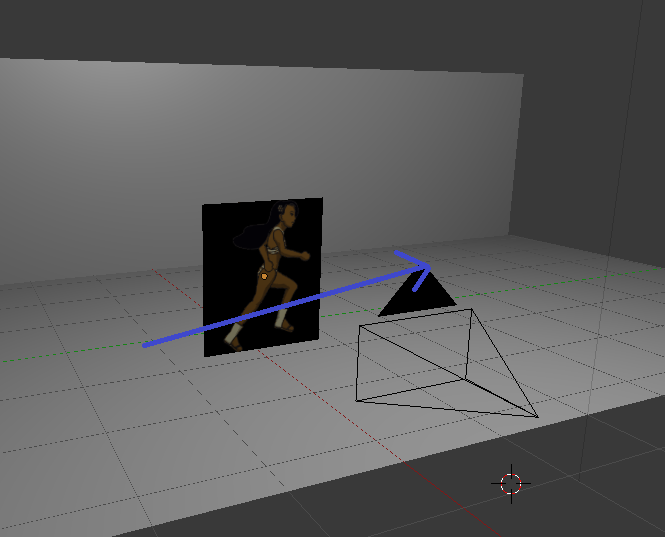
\includegraphics[width=0.7 \textwidth]{05TrabajoRealizado/01DocDiseno02/imagenes/camara01}}
   \subfigure[Seguimiento vertical.]{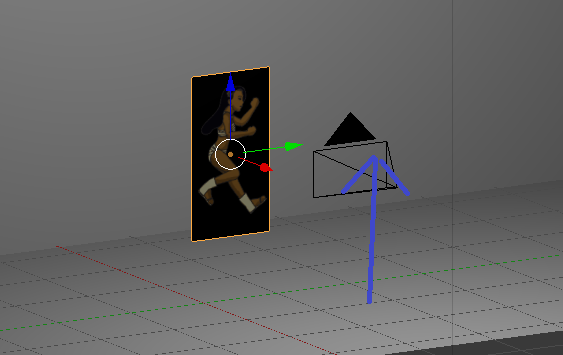
\includegraphics[width=0.7 \textwidth]{05TrabajoRealizado/01DocDiseno02/imagenes/camara02}}
  \caption{La cámara seguirá la posición del jugador en el eje x y y.}
  \label{fig:Camara}
\end{figure} 
 

\par
Por su parte, los controles del juego se establecieron como un conjunto de cuatro 
botones (Ver figura \ref{fig:GUI} ); cada uno con una acción específica a 
desempeñar: mover hacia la izquierda, mover hacia la derecha, disparar, hablar, 
saltar. Siendo periférico o el medio de interacción de los botones y el jugador 
la pantalla táctil del teléfono.  

\begin{figure}
				\centering
				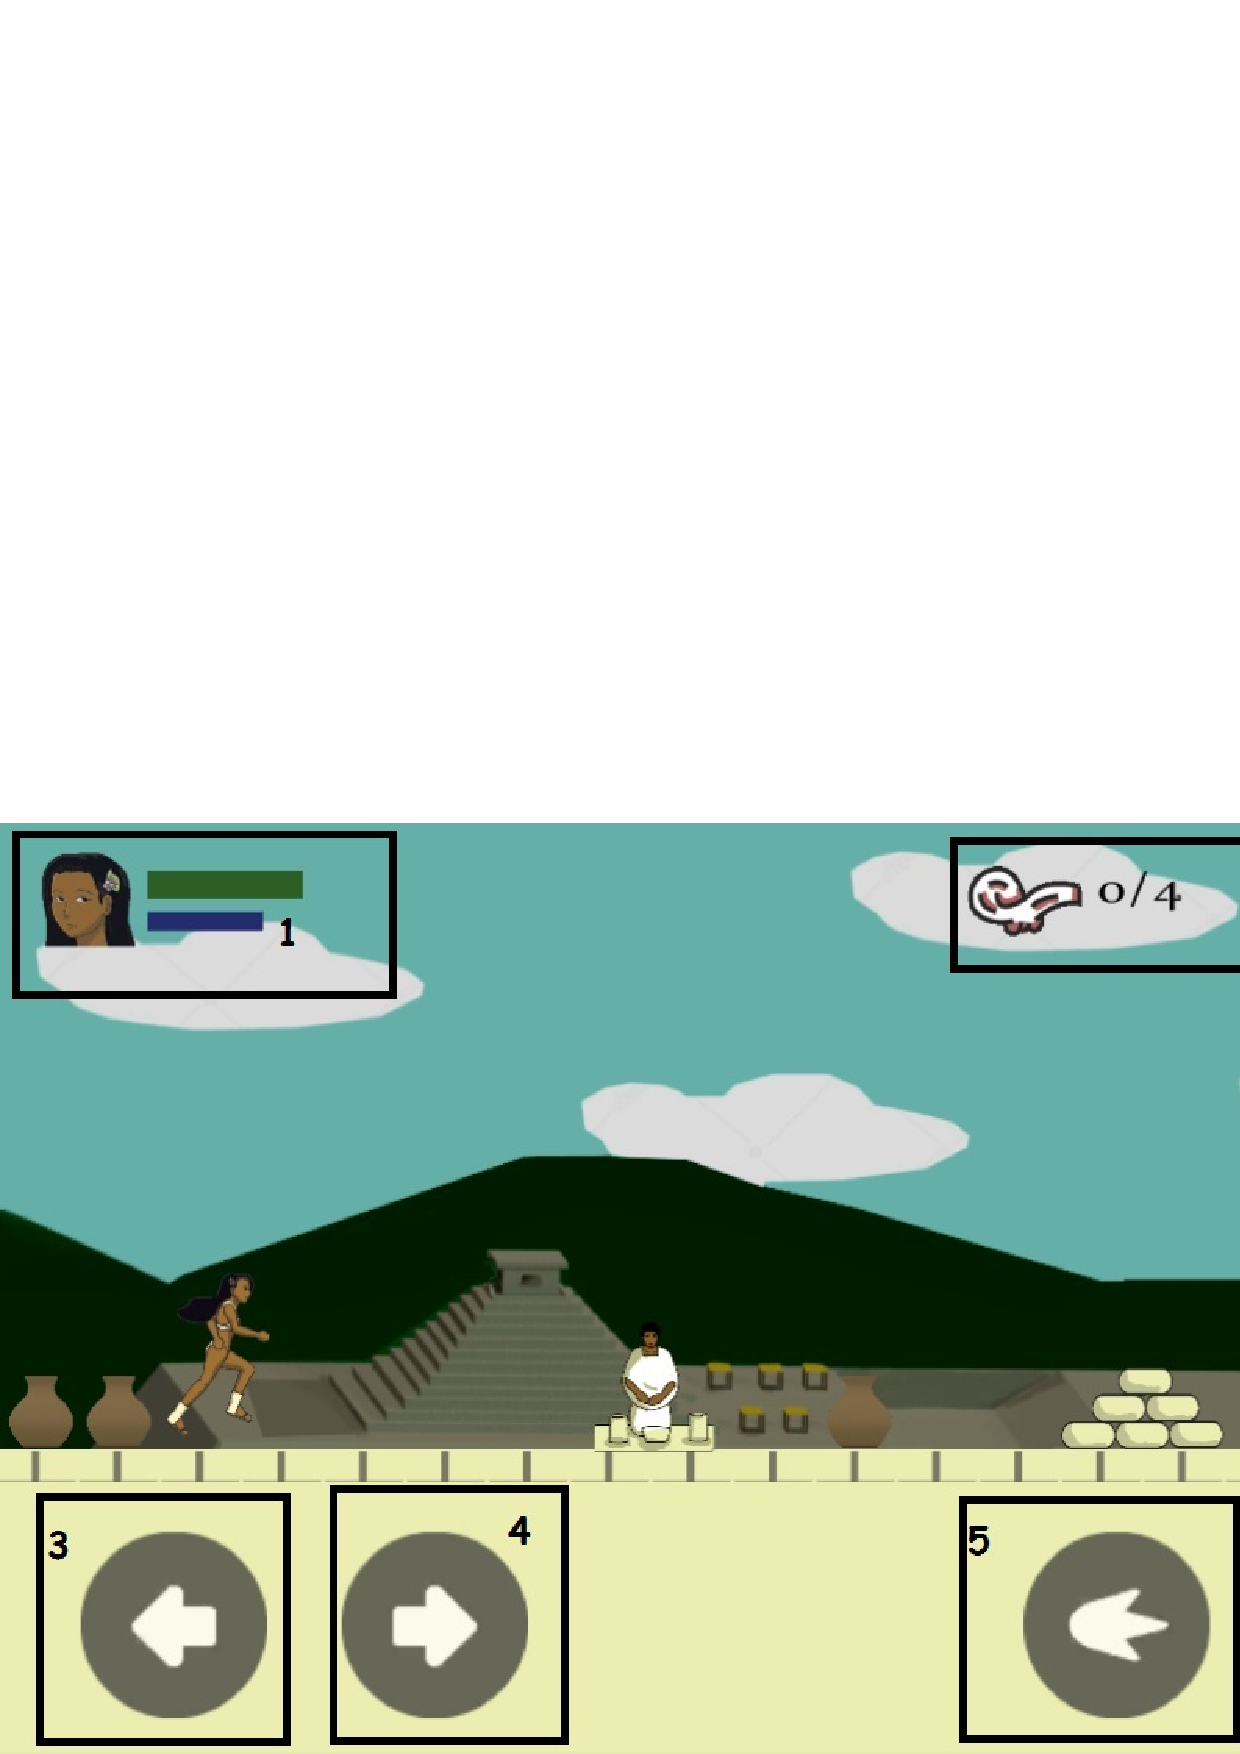
\includegraphics[height=0.3 \textheight]{05TrabajoRealizado/01DocDiseno02/imagenes/ControlCorrerDer}
				\caption{1 Información del personaje jugable, barra verde indicador 
				de la cantidad de vida, barra azul cantidad de tonalli. 2 Objetivos 
				del nivel o información útil. 3 Botón moverse izquierda. 4 Botón 
				moverse derecha. 5 Botón disparar tonalli. 6 Botón saltar.}
				\label{fig:GUI}
\end{figure}


\par
En cuanto al guardado y la carga, se propusieron dos tipos guardado y carga automática 
y guardado y carga de checkpoint; el primero guarda el progreso del jugador al 
completar el nivel y permite inicializar los niveles desbloqueados y el segundo 
se utiliza dentro de un nivel para guardar el progreso del jugador en el nivel 
en caso de que muera pueda iniciar desde el último checkpoint que tocó. 
Si el lector de este documento dese profundizar más en lo anteriormente dicho, 
se le recomienda consultar el Capítulo 5 del documento de diseño.
%===========================================
\subsection{Interfaces}\label{TraReaInterfaces}
Para la navegación dentro del juego, se diseñaron tres interfaces gráficas: 
La pantalla de inicio, Menú principal y el menú de selección de nivel. 
A continuación, se hará una breve descripción de la función principal de 
las interfaces:
\begin{itemize}
	\item\textbf{ Interfaz de inicio:} Presenta el logo del juego y la información 
	legal del mismo, sirve como pantalla de introducción al juego. Conecta con 
	la interfaz de menú principal (Ver figura \ref{fig:PInicio} ) .
	\item \textbf{Interfaz de menú principal:} Muestra la misma ilustración que la 
	pantalla de inicio, con la diferencia de que muestra dos botones en la parte 
	inferior izquierda de la pantalla. Con estos botones se puede empezar una nueva 
	partida o cargar una ya existente. Esta interfaz conecta a la cinemática de 
	inicio del juego si el jugador oprime el botón de empezar partida y confirma 
	que desea empezar una partida nueva o direcciona a la interfaz de menú de 
	selección de nivel, si el jugado oprime el botón de cargar partida y existe 
	un archivo con los datos del juego (Ver figura \ref{fig:PMenuP}).
	\item \textbf{Interfaz de Menú selección de nivel:} En esta interfaz el 
	jugador podrá elegir el nivel que desea jugar, siempre que lo haya desbloqueado 
	con anterioridad (Ver figura \ref{fig:SelNivel}).
\end{itemize}

\begin{figure}
  \centering
   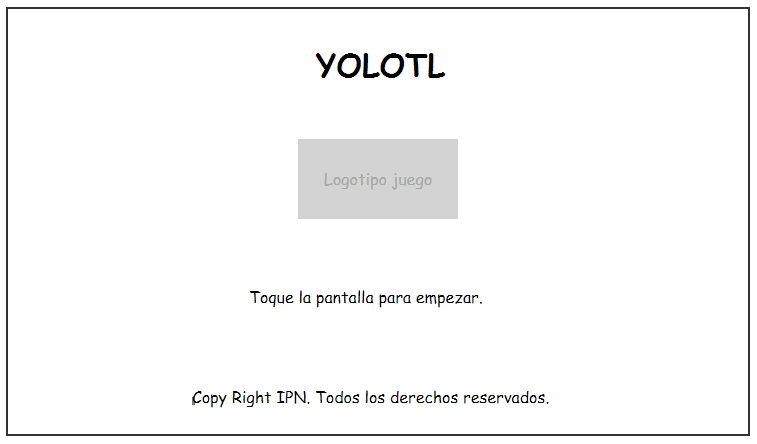
\includegraphics[width=0.6 \textwidth]{05TrabajoRealizado/01DocDiseno02/imagenes/interfaz00}
  \caption{Interfaz 1.0 Pantalla de inicio.}
  \label{fig:PInicio}
\end{figure} 


\begin{figure}
  \centering
   \subfigure[Menú principal] {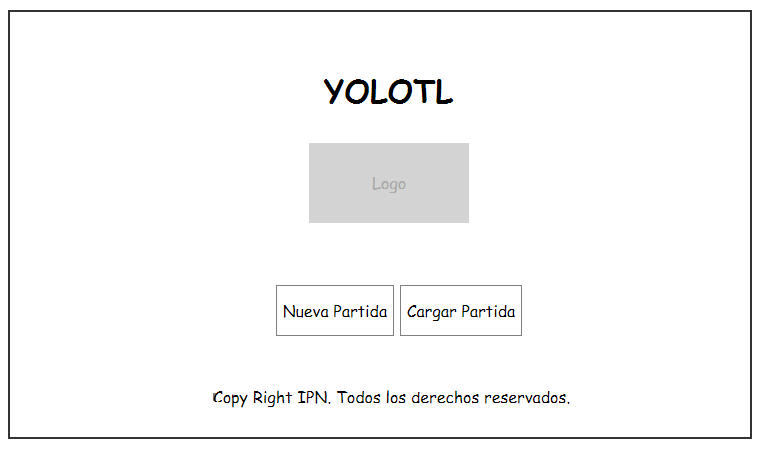
\includegraphics[width=0.6 \textwidth]{05TrabajoRealizado/01DocDiseno02/imagenes/interfaz01}}
   
 	\subfigure[Cuadro de dialogo para confirmar iniciar nueva partida.] {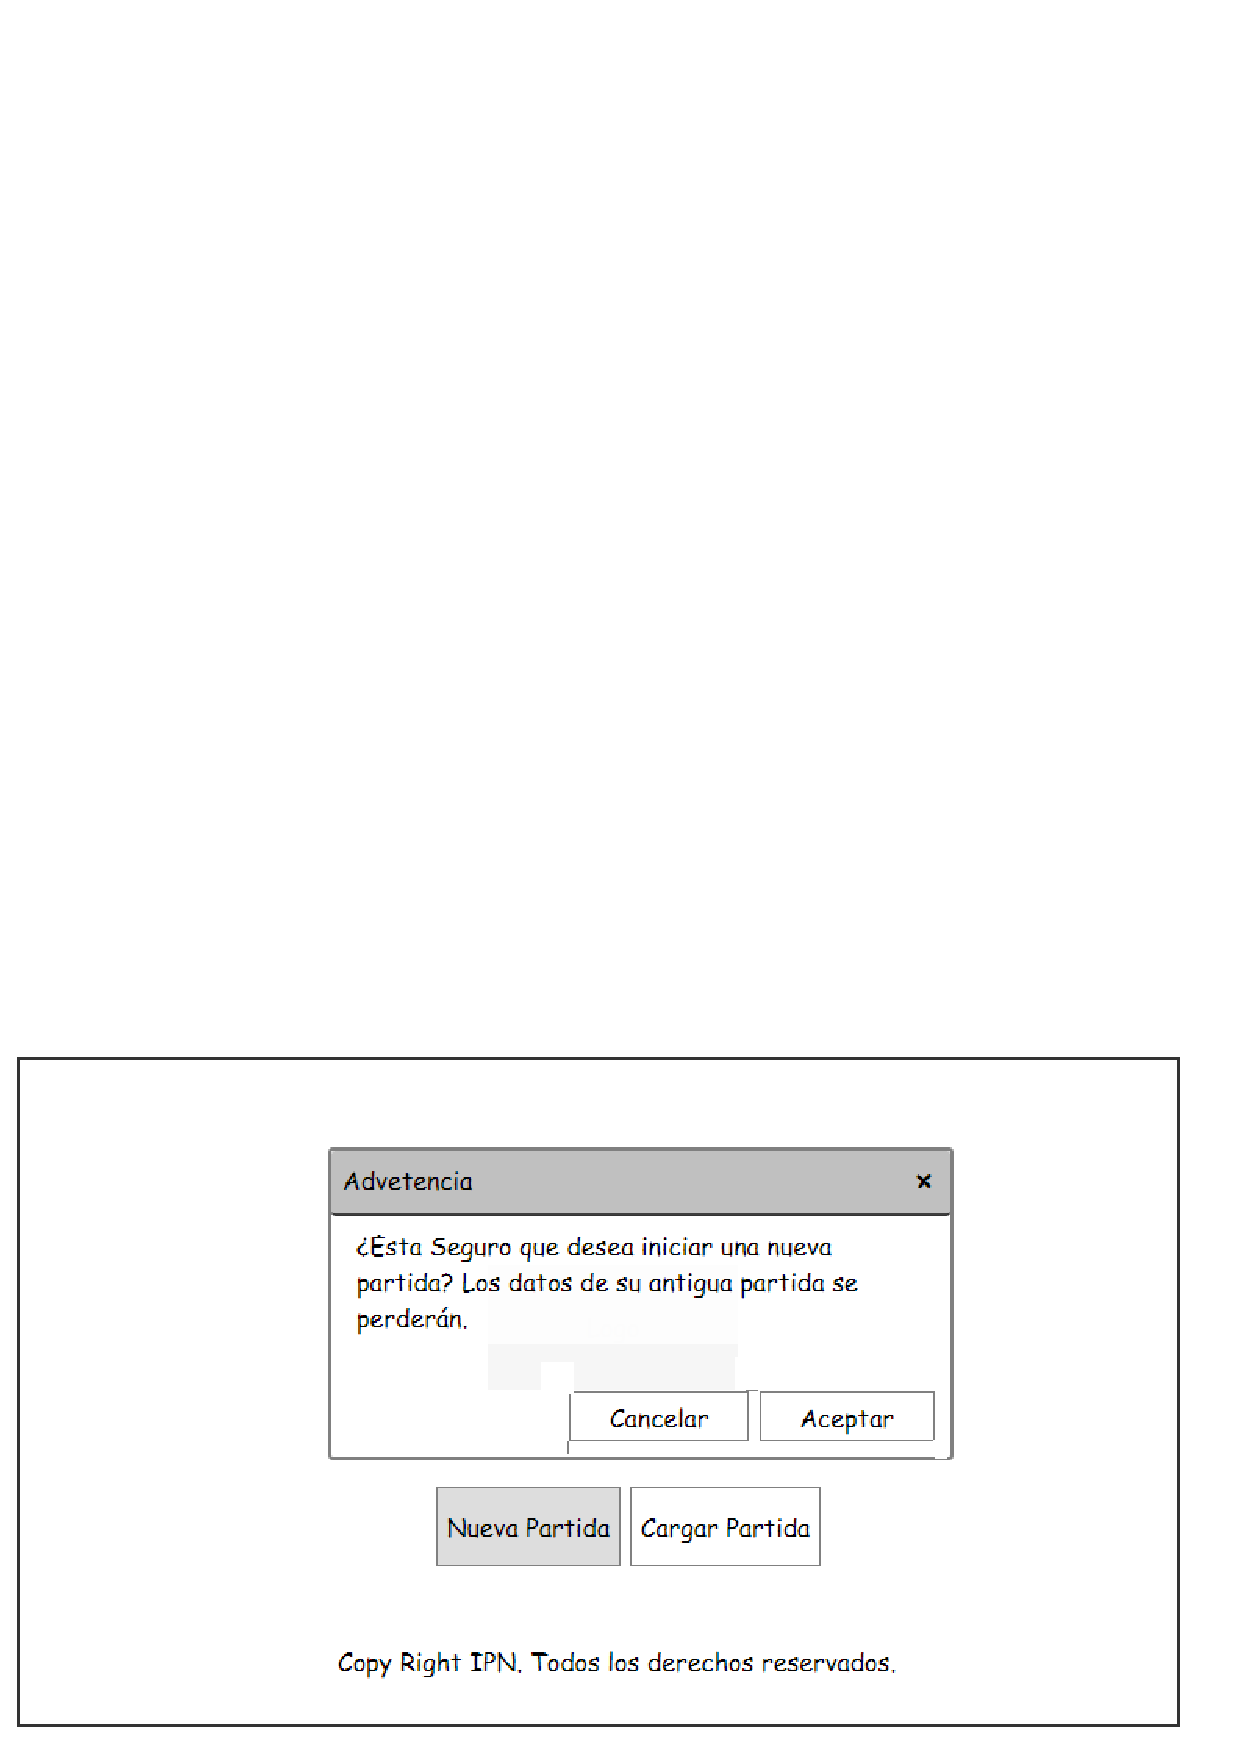
\includegraphics[width=0.6 \textwidth]{05TrabajoRealizado/01DocDiseno02/imagenes/interfaz01_02}}
 	
\subfigure[Cuadro de dialogo cuando no existen partidas que cargar.] {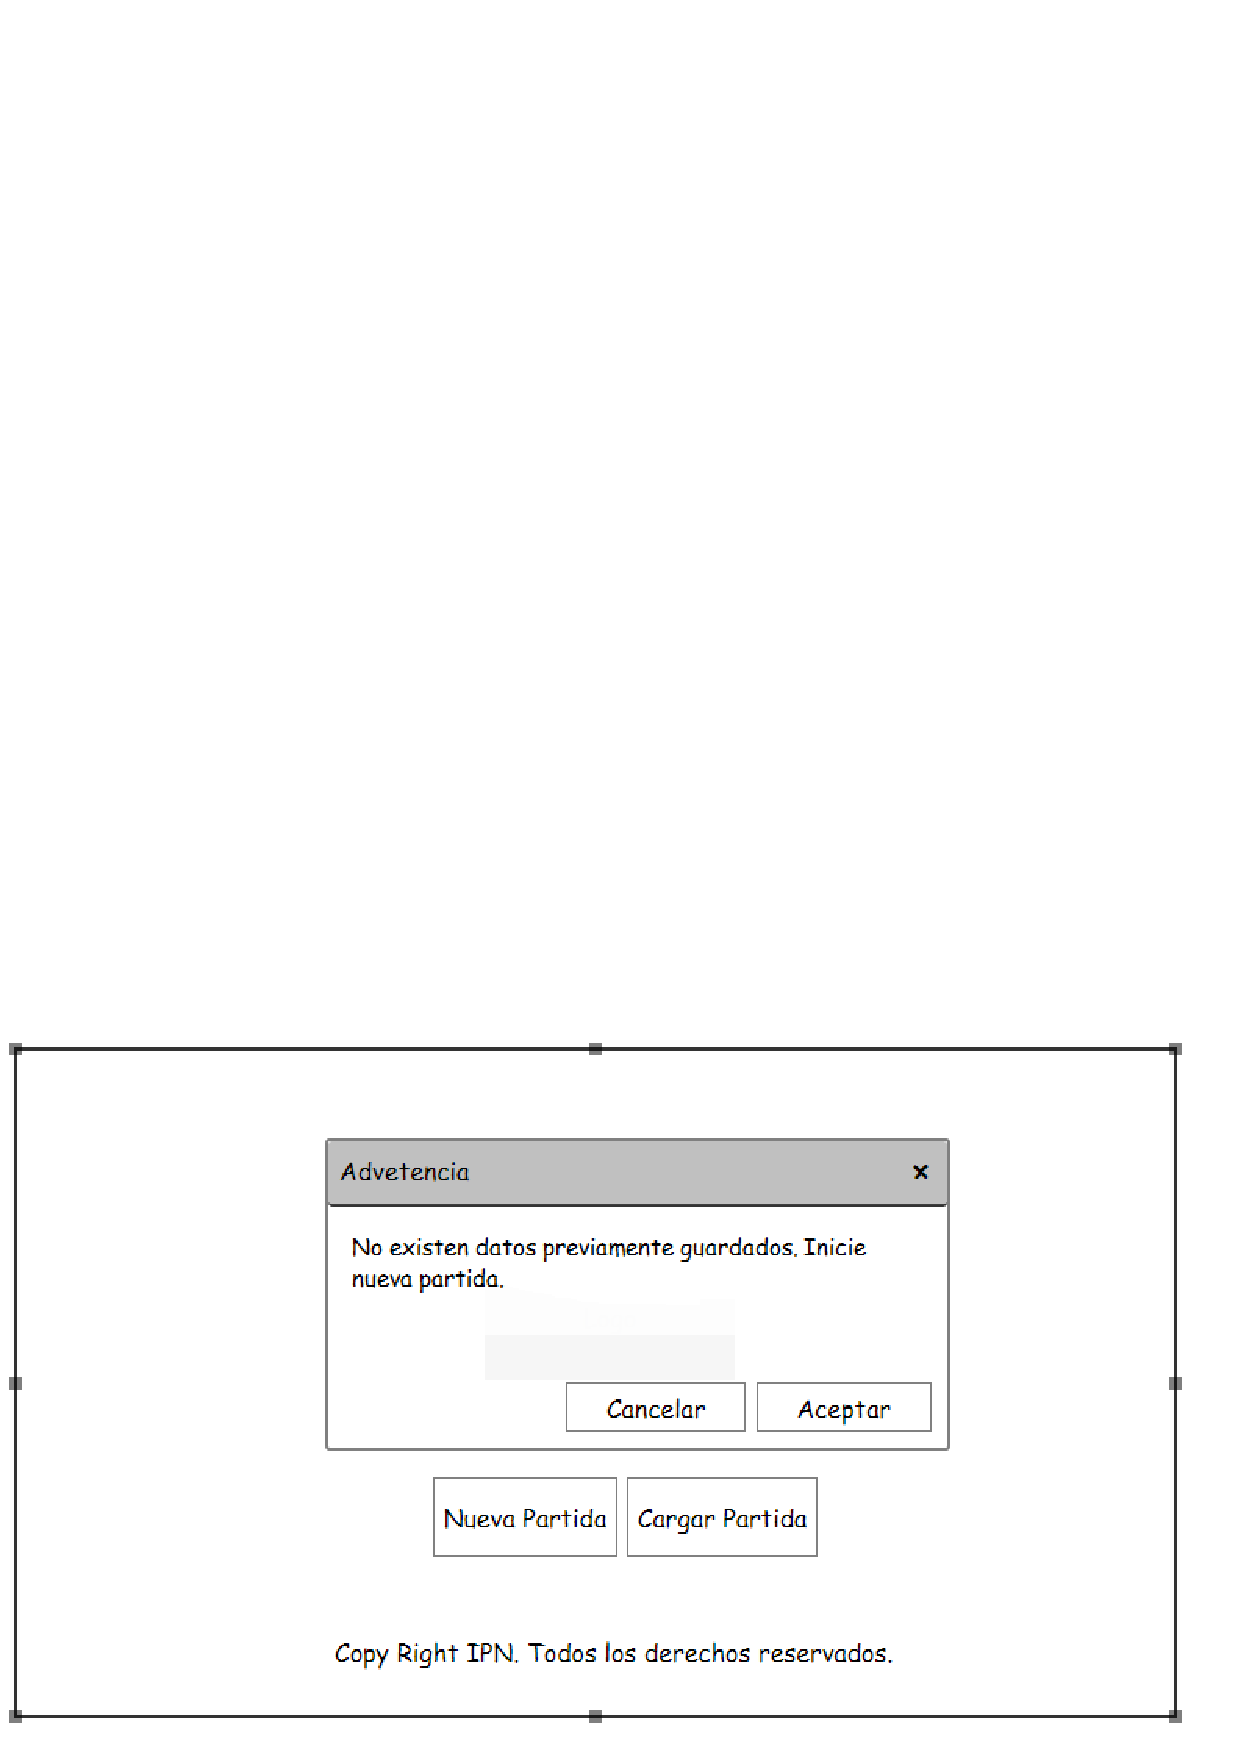
\includegraphics[width=0.6 \textwidth]{05TrabajoRealizado/01DocDiseno02/imagenes/interfaz01_03}}
  \caption{Interfaz 2.00 Menú principal.}
  \label{fig:PMenuP}
\end{figure} 


\begin{figure}
  \centering
   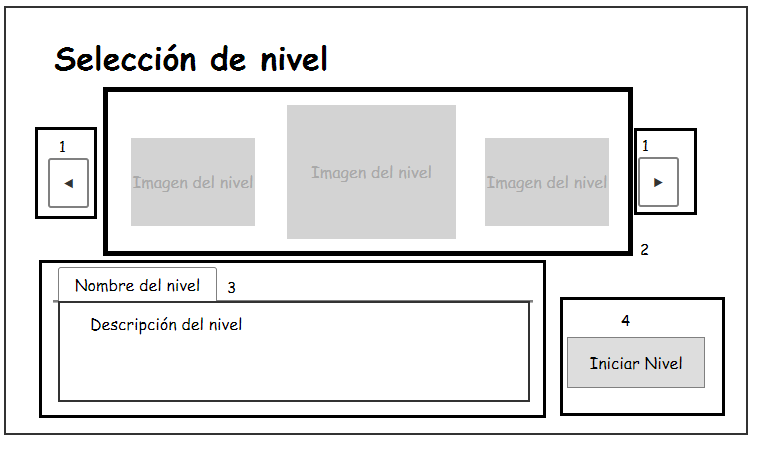
\includegraphics[width=0.6 \textwidth]{05TrabajoRealizado/01DocDiseno02/imagenes/interfaz02_01}
  \caption{Interfaz 2.00 Selección de nivel.1 botones que controlan el carrusel. 2 Carrusel. 3 Información del nivel seleccionado. 4 Botón Iniciar nivel.}
  \label{fig:SelNivel}
\end{figure}  
%===========================================
\subsection{Niveles.} \label{Niveles}
Yolotl es un juego compuesto por diez niveles: un nivel introductorio y los nueve 
niveles del inframundo.  Dado que la idea concepto del juego Yolotl lo situa en 
el Mictlán, la cantidad mínima esperados seria nueve; sin embargo, se tomó la 
decisión de incluir un nivel de introducción debido a los siguientes factores: 

\begin{itemize}
	\item Introducir al jugador a las mecánicas de juego básicas antes de lanzarlo 
	a un nivel más complicado.
	\item Situar el juego dentro de un contexto histórico real, permitiéndole al 
	jugador conocer sobre la sociedad Mexica de una manera en la que el jugador 
	pueda ser participe de este contexto histórico.
	\item Seguir una estructura narrativa básica en la que se presente la vida 
	cotidiana del héroe antes del llamado a la aventura \cite{RefHeroe}.
\end{itemize}

Usualmente, en el juego de Yolotl, un nivel está compuesto de dos secciones: una 
sección de obstáculos y plataformas en donde cumplirá un objetivo propio del nivel 
y otra donde el jugador se enfrentará al enemigo jefe del nivel. A excepción 
del primero y ultimo nivel el resto de los niveles siguen esa estructura. En el 
caso del primer nivel sigue la división de las dos secciones, con la diferencia 
de que no existe un enemigo jefe a vencer en la segunda sección del nivel; 
mientras que en el último nivel existe una única sección en donde el jugador 
se enfrentará a las diferentes transformaciones del jefe final.
\\
\par
La progresión entre niveles es lineal (Ver figura \ref{fig:ProgreNiveles}), 
por lo que no se puede acceder al nivel determinado sin antes haber completado 
a su predecesor; siendo el primer nivel, el que se encuentra disponible de manera 
estándar al empezar una nueva partida. Un nivel se da completado únicamente 
hasta que se ha derrotado al enemigo jefe del nivel; salvo por el primer nivel, 
el cual se considera terminado una vez que el jugador obtiene el arma de la 
protagonista. Cuando el jugador completa un nivel, además de desbloquear el 
siguiente nivel, el jugador podrá ver determinadas cinemáticas con las que podrá 
seguir la historia del juego y obtiene mejoras sobre alguno de los atributos del 
personaje.
\\
\par
En la tabla se encuentra información referente a cada nivel tal como los 
objetivos a cumplir, el enemigo a vencer, lo que se obtiene al completar el nivel.

%%============== PROGRECION DE NIVELES ==============
\begin{figure}
  \centering
   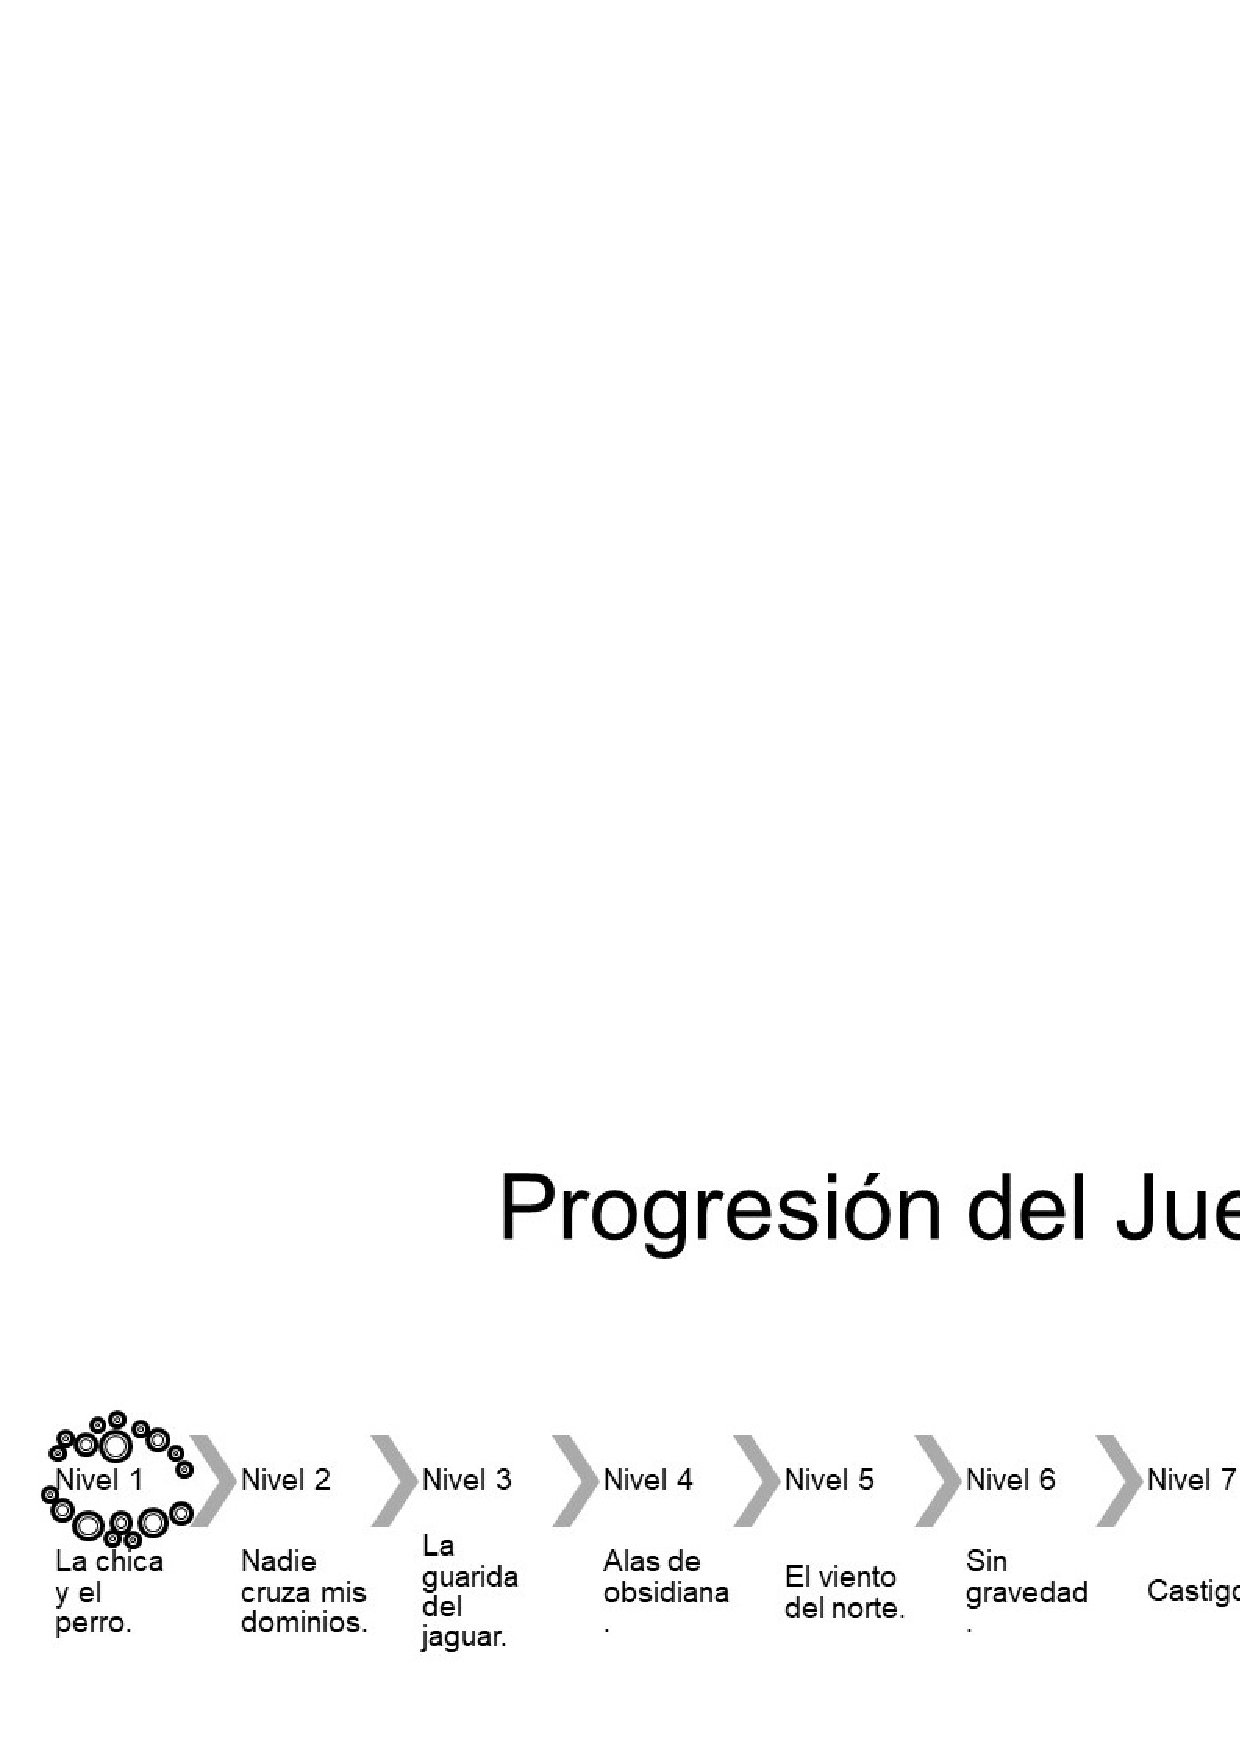
\includegraphics[width=0.8 \textwidth]{05TrabajoRealizado/01DocDiseno02/imagenes/ProgresJuego}
  \caption{Progresión del juego}
  \label{fig:ProgreNiveles}
\end{figure} 

%%============== TABLA DE NIVELES =============
%\begin{table}
	\begin{longtable}[c]{ | m{3.75cm} | m{3.75cm}| m{3.75cm} | m{3.75cm}|} 
		%\endhead		
		%\endfirsthead
		%\endlastfoot
		%\hline
		\rowcolor{cyan} Nivel.& Objetivo & Zona de plataformas	Enemigo jefe & Progreso obtenido. \\ 
		\hline
		%-------------------------------
		Nivel 1 “La chica y el perro”. & 
		Hablar con al menos cuatro ciudadanos.
			\par 
			Interactuar con Xólotl.
			\par 
			Obtener la caracola.&
		Sin enemigo jefe.&
		 Nivel 1.
			\par 
			Cinemática 3.
			\par 
			Cinemática 4.
			\par 
			Habilidad de disparo.		 
		 \\ 
		\hline
		%-------------------------------
		Nivel 2 “Nadie cruza mis dominios”. & 
		Atravesar el rio evitando tocar a los Xoloitzcuintles, por cada Xoloitzcuintles tocado incrementara el poder de Xochitónal. &
		Xochitónal. &
		Mejora en la cantidad de vida de Malinalli.
			\par 
			Cinemática 6.
			\par 
			Cinemática 7.
			\par 
			Cinemática 8.
			\par 
			Cinemática 9.
			\par 
			Cinemática 10.
			\par 
			Nivel 3.		 
		 \\ 
		\hline
		%-------------------------------
		Nivel 3 “La guarida del jaguar”. & 
		Llegar a la guarida de Tepeyóllotl. &
		Tepeyóllotl. &
		Mejora en la cantidad de Tonalli de Malinalli.
			\par 
			Cinemática 12.
			\par
			Cinemática 13.
			\par 
			Cinemática 14.
			\par
			Nivel 4.		 
		 \\ 
		\hline
		%-------------------------------
		Nivel 4 “Alas de obsidiana”. & 
			Encontrar el camino correcto hacia la guarida de Itzpapálotl.
			\par
			Encontrar las tres llaves que abren la puerta de la guarida de Itzpapálotl.&
		Itzpapálotl. &
			 Mejora en la cantidad de vida de Malinalli.
			 \par
			 Cinemática 16.
			 \par
			 Cinemática 17.
			 \par
			 Cinemática 18.
			 \par
			 Cinemática 19.
			 \par
			 Cinemática 20.
			 \par
			 Cinemática 21.
			 \par
			 Cinemática 22.
			 \par
			 Nivel 5.		 
		 \\ 
		\hline
		%-------------------------------
		Nivel 5 “El viento del norte”. & 
		Llegar a la guarida Mictlecayotl.&
		Mictlecayotl. &
		Mejora en la cantidad de Tonalli de Malinalli.
		\par
		Cinemática 24.
		\par
		Cinemática 25.
		\par
		Cinemática 26.
		\par
		Cinemática 27.
		\par
		Nivel 6.		 
		 \\ 
		\hline
		%-------------------------------
		Nivel 6 “Sin gravedad”. & 
		Llegar a la guarida Tlazoltéotl &
		Tlazoltéotl. &
		Mejora en la cantidad de vida de Malinalli.
		\par
		Cinemática 29.
		\par
		Cinemática 30.
		\par
		Cinemática 31.
		\par
		 Nivel 7.		 
		 \\ 
		\hline
		%-------------------------------
		Nivel 7 “Castigo”. & 
		Llegar a la guardia Itztlacoliuhqui. &
		Itztlacoliuhqui. &
		Mejora en la cantidad de Tonalli de Malinalli.
		\par
		Cinemática 33.
		\par
		Cinemática 34.
		\par
		Cinemática 35.
		\par
		Nivel 8.		 
		 \\ 
		\hline
		%-------------------------------
		Nivel 8 “La última batalla del jaguar”. & 
		Llegar a la guarida de Tepeyóllotl.&
		Tepeyóllotl. &
		Mejora en la cantidad de vida de Malinalli.
		\par		
		Cinemática 37.
		\par
		Cinemática 38.
		\par
		Cinemática 39.
		\par
		Nivel 9.		 
		 \\ 
		\hline
		%-------------------------------
		Nivel 9 “El último caballero del rey”. & 
		Superar la zona de Tula.
		\par
		Superar la zona de Oluta.&
		Nexoxcho. &
		Mejora en la cantidad de Tonalli de Malinalli.
		\par		
		Cinemática 44.
		\par
		Cinemática 45.
		\par
		Cinemática 46.
		\par
		Nivel 10. 
		 \\ 
		\hline
		%-------------------------------
		Nivel 10 “El rey del Mictlán”. & 
		Sin objetivos &
		Mictlantecutli. &
		Cinemática 47.
		\par		
		Juego terminado. 
		 \\ 
		\hline
	\end{longtable}

	%\caption{Información de los niveles.}
	%\label{Tab:Niveles}
%\end{table}
%===========================================
\subsection{Obstáculos}
De manera particular, para el proyecto Yolotl, se entiende por obstáculos a aquellos objetos dentro de un nivel que dificultan el avance continuo del jugado o que faciliten el fallo del jugador.
\\
\par
A diferencia de los personajes, la metodología huddle no maneja una plantilla para documentar estos objetos, por lo que se propuso una plantilla propia. Los campos de la plantilla son:
	\begin{itemize}
		\item Nombre del obstáculo.
		\item Descripción: Este campo describe tanto físicamente el objeto como su comportamiento e interacción con el jugador. 
		\item Esquema: Imagen de apoyo que facilita la comprensión de la descripción. 
	\end{itemize}
En total se definieron alrededor de 11 obstáculos, mismos que se podrán encontrar repartidos a lo largo de los niveles del juego. Algunos obstáculos serán exclusivos de un nivel mientras que otros se podrán encontrar en todos los niveles.
 \\
 \par
 A continuación se listarán los obstáculos del juego:
 	\begin{itemize}
 		\item Caja.
 		\item Sacos de cacao.
 		\item Plataforma móvil.
 		\item Plataforma que cae.
 		\item Plataforma que desaparece.
 		\item Estalagmitas.
 		\item Viento temporal.
 		\item Piedras filosas.
 		\item Piso congelado.
 		\item Bolas de nieve.
 		\item Lluvia de flechas.
 	\end{itemize}
%===========================================
\subsection{Ambientación}
	Para garantizar la inmersión del jugador, el videojuego se vale de diferentes
	 elementos multimedia. Estos elementos son la música de fondo (BGM, pos sus 
	 siglas en inglés), los efectos de sonido (SFX, por sus siglas en inglés) y  
	 efectos espaciales (FX, por su siglas en inglés).
\\
\par	
	Huddle maneja un aparatado para incluir este tipo de elementos dentro de la 
	documentación del juego; sin embargo, no incluye ninguna guía sobre como debería 
	de redactarse las descripciones de BGM y SFX; en consecuencia estos elementos 
	fueron documentados escribiendo el nombre de sonido o música, seguido de una 
	breve descripción del mismo.   
\\
\par
Durante la redacción de este aparatado se detectó que existían dos secciones para 
documentar BGM y SFX, con la diferencia de que en una los términos se encontraban 
escritos en sus siglas en inglés y en el otro apartado se encontraba en español, 
por lo que se eliminó el apartado en español. Luego de que se detectara esta 
duplicación de apartados, se descubrió que no existía ningún apartado para documentar 
los FX, seguido de esto se creo dicho apartado. En cuanto a la documentación de FX, 
se siguió la misma estructura que con BGM y SFX: escribir el nombre de FX y 
describirlo para dar una idea de como se vería en el nivel y bajo que interacciones 
se activaría. 
%===========================================
\subsection{Argumento del videojuego}
Huddle maneja un apartado llamado \textbf{Guión} para documentar de manera detallada 
la historia del videojuego. No obstante, al igual que como sucede con algunos de 
los apartados ya descritos, Huddle no proporciona una plantilla para documentarlo. 
Ante la falta de una plantilla para documentar el argumento y ante la existencia 
de cinemáticas dentro de los niveles y fuera de estos, se decidió que el argumento 
del juego se documentaría como una animación. Contando así con tres guiones:
	\begin{itemize}
		\item \textbf{Guión literario}:Este guión es parecido a un guión teatral. 
		Por medio de escenas va desarrollando la historia, mostrando la secuencia 
		de diálogos que entablan los personajes participes en el argumento. Para 
		el caso particular del videojuego Yolotl, las escenas recibe el nombre de 
		cinemáticas. Cada cinemática se documentara bajo la siguiente plantilla:
			\begin{itemize}
				\item Numero de la cinemática seguido del nombre la locación donde 
				acontece ésta; en caso de que la escena suceda en el interior de 
				alguna edificación se pondrá seguido del nombre de la locación el 
				prefijo int, en caso de suceder en el exterior se colocará el 
				prefijo ext.
				\item Relación con los nombres de todos los personajes que participan 
				en la escena.
				\item Breve descripción de la locación.
				\item Secuencia de diálogos. Cada diálogo va precedido por el nombre 
				de personaje que lo dice, el nombre del personaje debe de ir en 
				mayúsculas y subrayado. 
			\end{itemize}
			\item Storyboard: El storyboard es una secuencia de imágenes que narran 
			de manera visual la historia. Cada imagen va comentada de tecnicismos 
			que faciliten la descripción de acciones (tales como el desplazamiento 
			de la cámara, movimientos de personajes, intención del personaje en 
			decir un diálogo, etc.) \cite{RefStoyBoard}.  			 
	\end{itemize}

